% ============================================================
% Appendix: supplementary material moved out of the main text for length.
% Each section here was relocated from the main paper; the original location
% retains a short summary + a "% MOVED TO APPENDIX" marker for traceability.
% ============================================================

\section{Search Quality vs.\ a Uniform-Route Exhaustive Oracle}
\label{sec:eval_oracle}
% (Moved from the Evaluation section.)

To assess whether state-guided candidate pruning misses significantly better configurations, we compare SWEEP-LLM's decisions against a \emph{uniform-route} exhaustive oracle that uses the same common $\rho$-gate and power model.
The oracle is exhaustive over the pool-bundle and frequency space (no state-guided pruning): it evaluates all valid PoolBundle combinations for both pools (${\approx}25{\times}70$ bundle pairs), all ten frequency levels per pool, and the four routes (AA, AB, BA, BB), yielding ${\approx}44{,}000$ candidates per window.
It applies a \emph{single} route to the whole window, however, rather than enumerating per-class route maps; it therefore searches a different space than SWEEP-LLM, which additionally selects a route per class (up to $4^{K}$ maps). The oracle is thus a search-quality reference over the bundle/frequency space, not a global optimum over SWEEP-LLM's full decision space, and on windows where per-class routing helps SWEEP-LLM can match it despite searching far fewer candidates.

Table~\ref{tab:oracle_gap} reports results across seven representative windows spanning all four workload states at relevant operating rates.

\begin{table}[!t]
\centering
\caption{Energy gap between SWEEP-LLM and a uniform-route exhaustive oracle (exhaustive over bundles and frequencies, single route per window); all windows feasible under the common $\rho$-gate.}
\label{tab:oracle_gap}
\small
\begin{tabular}{llrrr}
\toprule
Window & State & Rate & SWEEP (J) & Gap\% \\
\midrule
Balanced BOTH\_LOW & BOTH\_LOW & 6\,rps & 828.5 & 0.1\% \\
Prefill-heavy & PREFILL\_HEAVY & 20\,rps & 1638.0 & 6.8\% \\
Balanced high & BOTH\_HEAVY & 30\,rps & 2741.5 & 5.0\% \\
Prefill-heavy (high) & PREFILL\_HEAVY & 25\,rps & 2131.5 & 12.3\% \\
Biased BOTH\_LOW (PF) & BOTH\_LOW & 5\,rps & 828.5 & 25.4\% \\
Biased BOTH\_LOW (DC) & BOTH\_LOW & 5\,rps & 868.0 & 28.8\% \\
Decode-heavy & DECODE\_HEAVY & 30\,rps & 2295.0 & 0.0\% \\
\bottomrule
\end{tabular}
\end{table}

In the states where SLO constraints are most binding—PREFILL\_HEAVY and BOTH\_HEAVY—SWEEP-LLM is within 5--12\% of the oracle while running 5--35$\times$ faster.
For DECODE\_HEAVY and balanced BOTH\_LOW windows, SWEEP matches the oracle within 0.1\%.
The remaining gaps (25--29\%) occur in light-but-biased BOTH\_LOW windows, where the oracle exploits partial GPU allocations (e.g.\ 1--2 active GPUs) outside SWEEP's BOTH\_LOW candidate budget; the absolute energy difference in these low-load regimes is 168--194\,J.
Crucially, SWEEP-LLM \emph{never} misses a feasible configuration that the oracle finds: in all tested windows, SWEEP meets SLO whenever the oracle also meets SLO.


\section{Diurnal Robustness (1-week-derived)}
\label{sec:prod_diurnal}
% (Moved from the Production Traces section.)

The conv and code replays span only $7$--$12$ five-minute provisioning blocks, so DualScale-Ext's $5$-minute coarse tier sees relatively few reconfigurations. To test whether DualScale-Ext's under-provisioning is merely a short-trace artifact, and to evaluate all schedulers on a longer non-stationary segment, we extract a deterministic three-hour trough-to-peak segment from the one-week Azure conversation trace ($2024$-$05$-$12$\,$04{:}00$\,UTC, $234{,}038$ native requests, peak $21.7$\,rps) and deterministically thin it to $5/7/8.5$\,rps targets ($50/70/85\%$ of the Static-Disagg feasible peak), preserving the native time axis so the diurnal ramp is intact. Each replay spans $36$ five-minute blocks.

\begin{table}[t]
\centering
\caption{Diurnal robustness: 1-week-derived $3$\,h trough-to-peak conversation segment ($36$ five-minute blocks). Energy (kJ) and modeled violation (\%v) at $50/70/85\%$ of the Static-Disagg feasible peak.}
\label{tab:prod_diurnal}
\small
\setlength{\tabcolsep}{5pt}
\begin{tabular}{@{}lrrr@{}}
\toprule
Strategy & 50\% (kJ/\%v) & 70\% (kJ/\%v) & 85\% (kJ/\%v) \\
\midrule
Static-Disagg        & 14461 / 0.0 & 14781 / 0.0 & 15020 / 0.0 \\
GreenLLM-OracleDVFS  & 9432 / 0.0  & 10045 / 0.0 & 10423 / 0.0 \\
DynamoLLM-Mono       & 5314 / 0.0  & 5129 / 0.1  & 5348 / 7.0 \\
DualScale-Ext        & 3345 / 17.6 & 4135 / 23.9 & 4736 / 23.2 \\
Hierarchical-Disagg  & 4204 / 0.0  & 5363 / 0.0  & 6093 / 0.0 \\
\textbf{SWEEP-LLM}   & \textbf{4021 / 0.0} & \textbf{4269 / 0.0} & \textbf{4571 / 0.0} \\
\bottomrule
\end{tabular}
\end{table}

Three findings emerge from Table~\ref{tab:prod_diurnal}. First, \textbf{SWEEP-LLM is the lowest-energy $0\%$-violation scheduler at every load}, saving $4.3\%/20.4\%/25.0\%$ over Hierarchical-Disagg (the best feasible non-SWEEP baseline at each load). The savings grow monotonically with load: at light load both schedulers converge to similar operating points, while at higher load SWEEP-LLM's joint search exploits cross-pool routing and TP shapes the sequential greedy baseline cannot reach---consistent with the synthetic-trace ablation (Table~\ref{tab:ablation}).

Second, \textbf{DualScale-Ext under-provisions at every load} ($17.6\%/23.9\%/23.2\%$ modeled violation) even though the trace spans $36$ provisioning blocks. The coarse tier provisions for the peak observed in the trailing block, which is consistently below the next block's peak on a rising ramp---so its locked placement is always one block behind actual demand. This confirms the under-provisioning observed in the conv replay (Table~\ref{tab:prod_conv}) is a \emph{structural} limitation of fixed-cadence two-tier control on non-stationary traffic, not a short-trace artifact.

Third, at $85\%$ load \textbf{DualScale-Ext's $4736$\,kJ is actually higher than SWEEP-LLM's $4571$\,kJ}, despite its $23.2\%$ violations. At high load the locked placement cannot match SWEEP-LLM's joint search even when it is allowed to violate SLOs: the under-provisioned configuration runs the active GPUs harder and longer than SWEEP-LLM's correctly-sized one. DynamoLLM-Mono is feasible at $50/70\%$ ($0.0\%/0.1\%$) but degrades at $85\%$ ($7.0\%$), as monolithic routing forces over-aggregation under the peak.


\section{Idle-Power Sensitivity}
\label{sec:eval_idle}
% (Moved from the SLO Sensitivity section.)

We sweep the powered-idle GPU assumption over $P_{\mathrm{idle}}^{\mathrm{L40S}}/P_{\mathrm{idle}}^{\mathrm{L4}} \in \{0/0,\,45/9,\,90/18,\,150/30\}$\,W (zero, low, baseline, high).
Five of the six schedulers---Static-Disagg, GreenLLM-OracleDVFS, DualScale-Ext, Hierarchical-Disagg, and SWEEP-LLM---are completely insensitive ($0.0\%$ energy change from zero to high idle on every trace): each either keeps all active GPUs utilized or fully deactivates unused pools, so powered-idle GPUs never enter the energy calculation.
Only DynamoLLM-Mono is sensitive, and only on T3 and T4, where its monolithic routing leaves one pool partially idle across scheduling windows.
On T4, DynamoLLM-Mono's energy rises from $403$\,kJ at zero idle to $481$\,kJ at the baseline setting---widening SWEEP-LLM's advantage from $29\%$ to $41\%$---then falls to $467$\,kJ at high idle as it consolidates more aggressively to avoid the idle cost (a $39\%$ gap); on T3 the effect is small ($+1.5\%$, $328{\to}333$\,kJ).
SWEEP-LLM holds at $285$\,kJ (T4) and $319$\,kJ (T3) across all idle settings.


\section{Interconnect-Cost ($\tau_{kv}$) Sensitivity}
\label{sec:eval_taukv}
% (Figure moved from the synthetic-trace section.)

Cross-pool routes (A$\to$B and B$\to$A) add a KV-cache transfer term $\tau_{kv}\cdot\mathrm{il}$ to TTFT, where $\tau_{kv}$ is the per-token transfer cost and $\mathrm{il}$ is the prompt length (\S\ref{sec:eval_setup}). To test how sensitive SWEEP-LLM's energy is to the assumed interconnect speed, we sweep $\tau_{kv}\in\{5,16,41\}\,\mu$s/tok---representative of InfiniBand HDR, PCIe~4.0 with NCCL overhead, and 25\,GbE---at all three SLO levels on all four synthetic traces.

Figure~\ref{fig:section42_tau_kv} shows that total energy is essentially invariant to $\tau_{kv}$: the curves are flat at every SLO level, with a relative spread of $0.00\%$ across the swept range. Two effects explain this. First, the main cross-strategy comparison admits configurations through the common $\rho$-gate, which screens phase \emph{utilization} ($\rho\le1$) rather than latency; because $\tau_{kv}$ enters only the TTFT term and not utilization, it does not change the feasible set or the selected minimum-energy configuration. Second, the absolute transfer time is at most tens of milliseconds for the longest synthetic prompts (even at $\tau_{kv}{=}41\,\mu$s/tok), so even a latency-aware gate would see little movement in this range. The energy results of \S\ref{sec:eval_synth} are therefore robust to the interconnect-speed assumption across the practical fabric range; a deployment with a much slower interconnect or much longer prompts would place more weight on TTFT, which a latency-based admission gate would capture.

\begin{figure}[!t]
    \centering
    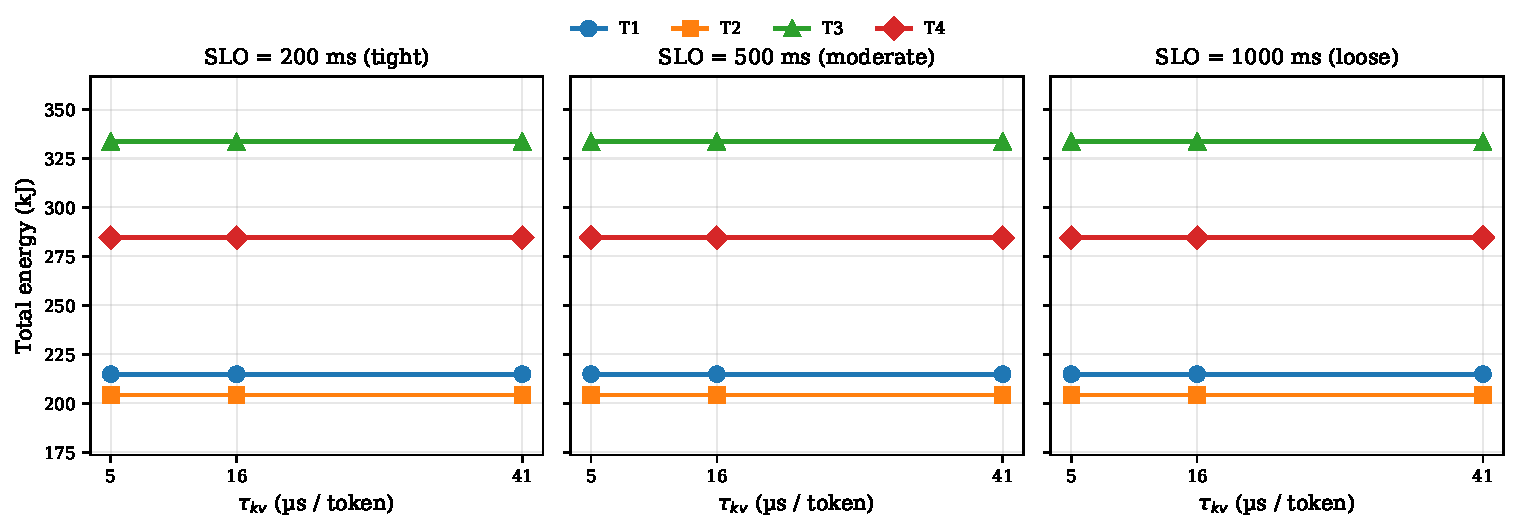
\includegraphics[width=\columnwidth]{figures/section42/tau_kv_sensitivity.pdf}
    \caption{SWEEP-LLM total energy versus the assumed cross-pool KV-transfer cost $\tau_{kv}$, at the three SLO levels. The $\tau_{kv}$ values are introduced in \S\ref{sec:eval_setup}. Under the common $\rho$-gate the curves are flat (relative spread $0.00\%$): the gate screens utilization, not latency, so the assumed fabric speed does not change the chosen configuration in the tested range.}
    \label{fig:section42_tau_kv}
\end{figure}


\section{Two-Tier Provisioning Cadence Sweep}
\label{sec:cadence_detail}
% (Table + detailed prose moved from the Cadence Sensitivity subsection; the main text keeps a summary.)

We sweep DualScale-Ext's coarse interval over $\{20\,\text{s}, 1, 2, 5\}$\,min (the $20$\,s setting is an aggressive cadence reported as an upper bound, not faithful to the paper) at the representative setting (SLO=500\,ms, $\tau_{kv}{=}16\,\mu$s/tok), using the same runner and windowizer as Table~\ref{tab:section42_main} so the numbers are directly comparable.

\begin{table}[t]
\centering
\caption{DualScale-Ext energy (kJ) and modeled violation (\%v) versus coarse provisioning cadence, against SWEEP-LLM (SLO=500\,ms, $\tau_{kv}{=}16\,\mu$s/tok).}
\label{tab:cadence}
\small
\setlength{\tabcolsep}{4pt}
\begin{tabular}{@{}lrrrrr@{}}
\toprule
 & \multicolumn{4}{c}{DualScale-Ext cadence (kJ / \%v)} & SWEEP \\
\cmidrule(lr){2-5}
Trace & 20\,s & 1\,min & 2\,min & 5\,min & kJ / \%v \\
\midrule
T1 & 218 / 35.8 & 226 / 40.8 & 236 / 39.2 & 167 / 44.2 & 215 / 0.0 \\
T2 & 190 / 12.5 & 193 / 16.7 & 197 / 24.2 & 165 / 39.2 & 192 / 0.0 \\
T3 & 305 / 28.3 & 297 / 37.5 & 301 / 31.7 & 286 / 68.3 & 319 / 0.0 \\
T4 & 234 / 41.7 & 382 / \phantom{0}3.3 & 383 / \phantom{0}4.2 & 402 / \phantom{0}0.8 & 285 / 0.0 \\
\bottomrule
\end{tabular}
\end{table}

Table~\ref{tab:cadence} shows that \emph{no} DualScale-Ext cadence reaches $0\%$ modeled
violations on any trace---the minimum anywhere is $0.8\%$ (T4 at $5$\,min). Every
configuration cheaper than SWEEP-LLM (e.g.\ T1/T2/T3 at $5$\,min, $165$--$286$\,kJ) carries
$28$--$68\%$ modeled violations: shorter cadences reduce some over-provisioning but still
under-provision ramping and bursty windows, while longer cadences appear energy-efficient
only by accepting high violation rates. In this cadence comparison SWEEP-LLM is the only
$0\%$-violation point, and it stays on the feasible energy frontier without depending on a
fixed coarse interval, because it re-evaluates placement every window while gating slow
actuation. (Static-Disagg, GreenLLM-OracleDVFS, and Hierarchical-Disagg are also $0\%$ but
at substantially higher energy; Table~\ref{tab:section42_main}.)


\section{Synthetic Trace Profiles}
\label{sec:synth_traces_appendix}
% (Figure moved from the synthetic-trace evaluation subsection.)

The four synthetic traces are $600$-second request streams replayed at $W{=}5$\,s windows, each constructed to exercise a different region of the window-state space defined in \S\ref{sec:window_classifier}. \textbf{T1} and \textbf{T2} are bell-shaped arrival ramps with, respectively, a prefill-heavy and a decode-heavy class mix; they sweep load while holding phase imbalance fixed and concentrate PREFILL\_HEAVY and DECODE\_HEAVY windows. \textbf{T3} holds the arrival rate constant while transitioning the class mix from the prefill-heavy mix of T1 to the decode-heavy mix of T2 at the trace midpoint, forcing an explicit state change without a confounding rate change. \textbf{T4} alternates between a baseline and a burst arrival rate over a balanced class mix, providing the BURST-flag coverage and most of the BOTH\_LOW and BOTH\_HEAVY windows.

Figure~\ref{fig:synth_traces} shows the per-window arrival rate, request-class composition, and assigned state for each trace; the realized rate, class mix, and state distribution match this design intent (verified with the classifier of \S\ref{sec:window_classifier}).

\begin{figure*}[!t]
    \centering
    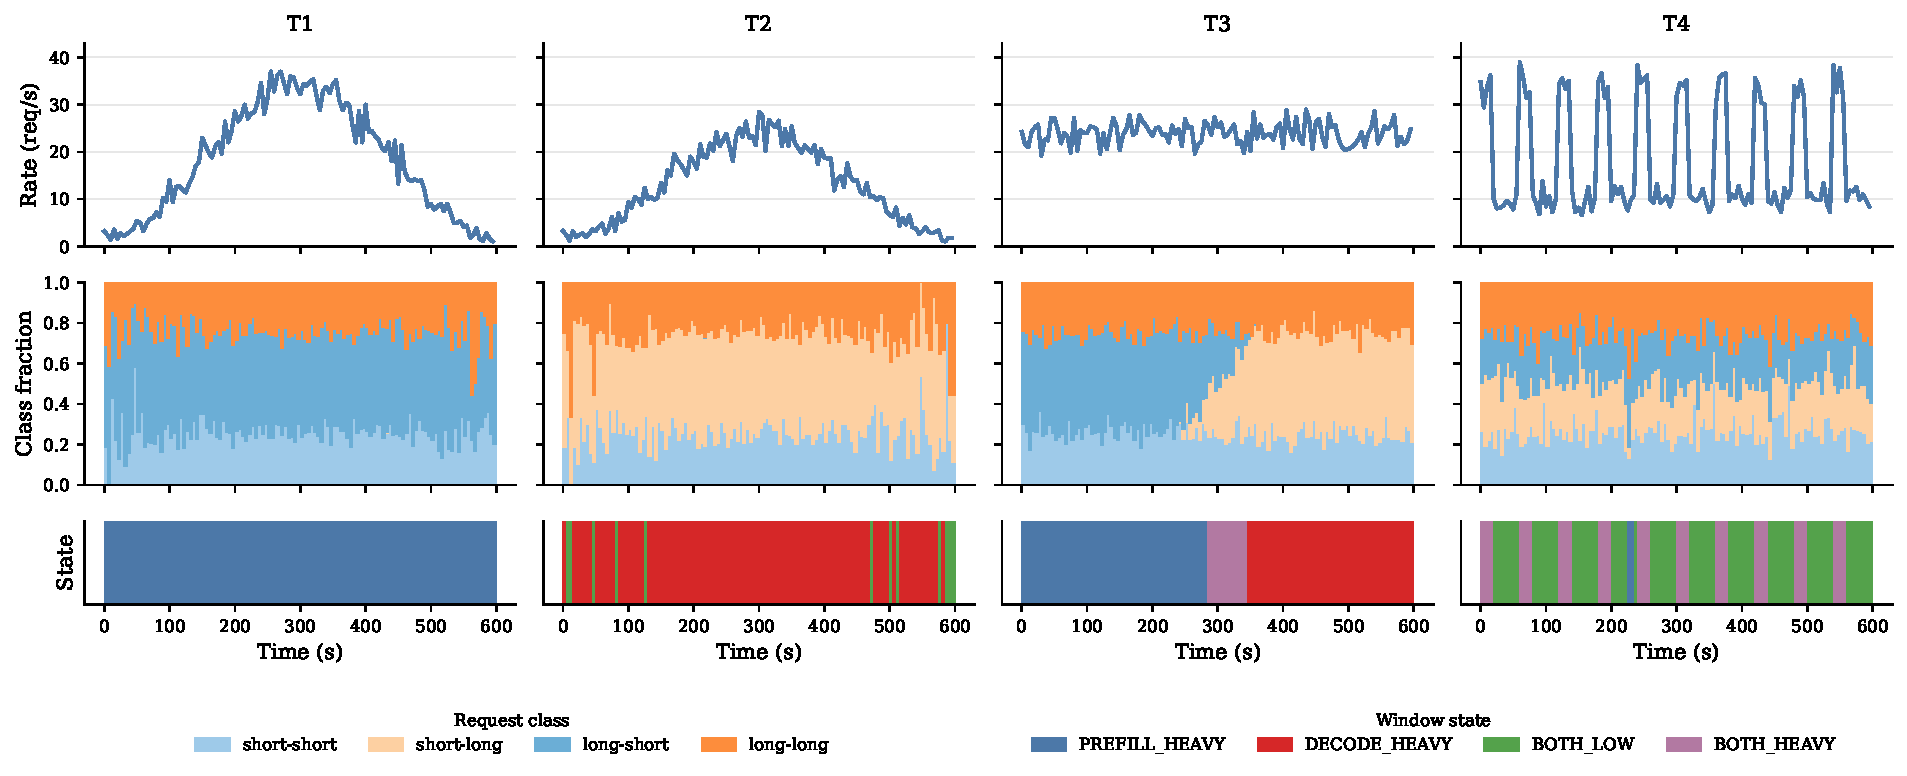
\includegraphics[width=\textwidth]{figures/section42/synthetic_trace_overview.pdf}
    \vspace{-0.8cm}
    \caption{Per-window arrival rate (top), request-class composition (middle), and assigned workload state (bottom) for the four synthetic traces. T1 and T2 are bell-shaped ramps with prefill- and decode-heavy mixes; T3 holds a constant rate while the class mix transitions through the trace midpoint; T4 alternates between baseline and burst rate over a balanced class mix.}
    \label{fig:synth_traces}
\end{figure*}


\section{Request-Class Granularity}
\label{sec:k_sensitivity}

We compare the default four-class ($2{\times}2$) taxonomy against a finer nine-class ($3{\times}3$) short/medium/long partition of input and output length on three length-diverse traces, holding all other settings fixed. Table~\ref{tab:k_sensitivity} reports total window energy, modeled violation rate, and per-run scheduler search time.

Refining to nine classes never improves energy at equal feasibility. On the two traces where it remains feasible ($0\%$ modeled violations), it uses $2.0$--$4.4\%$ \emph{more} energy than the four-class design. On the diurnal trace it reaches $2.2\%$ lower energy, but only by admitting $16.7\%$ modeled violations (versus $0\%$ for four classes), so it is not a valid operating point. Meanwhile, the per-window route search becomes $1.3$--$2.9\times$ more expensive, because the route-completion search branches per class. The four-class taxonomy therefore captures the available routing fidelity without the feasibility risk or the search-cost growth of a finer partition.

\begin{table}[t]
\centering
\small
\caption{Request-class granularity: four-class ($2{\times}2$) vs.\ nine-class ($3{\times}3$). ``Viol.''~is the modeled $\rho$-gate violation rate; ``Search''~is per-run scheduler time.}
\label{tab:k_sensitivity}
\begin{tabular}{@{}llrrr@{}}
\toprule
Trace & Scheme & Energy (kJ) & Viol.\ (\%) & Search (s) \\
\midrule
steady  & $2{\times}2$ & 11.35 & 0.0 & 146.9 \\
        & $3{\times}3$ & 11.85 & 0.0 & 421.8 \\
\midrule
bursty  & $2{\times}2$ & 18.45 & 0.0 & 60.2 \\
        & $3{\times}3$ & 18.81 & 0.0 & 78.2 \\
\midrule
diurnal & $2{\times}2$ & 22.77 & 0.0 & 104.3 \\
        & $3{\times}3$ & 22.26 & 16.7 & 236.5 \\
\bottomrule
\end{tabular}
\end{table}
